\chapter{الحركية المعقدة: السلاسل والإنزيمات والتذبذبات}\label{ch:b3:complex-kinetics}

كأس من محلول يُحرَّك يصير عديم اللون، ثم كهرمانيًا، ثم أزرق، ثم
عديم اللون من جديد، ويستمر على ذلك دقائق كثيرة؛ وإذا صُبّ في طبق رسم
الخليط نفسه حلزونات تدور وتنتقل. وحين وصف بوريس بيلوسوف
تفاعلًا كهذا سنة 1951، رُفضت مخطوطته: فقد رأى المحكّم أن النظام الكيميائي
لا يمكن أن يذهب ويجيء، لأنه يجب أن ينحدر
نحو التوازن. وهو ينحدر فعلًا؛ لكنه لا ينحدر
في خط مستقيم. يعالج هذا الفصل آليات ذات خطوات كثيرة تُجدَّد وسائطها:
\omterm{def:b3:complex-kinetics:chain}{التفاعلات المتسلسلة} والانفجارات، والجزيئات التي تحتاج إلى
تصادمات كي تتفكك وحدها، والإنزيمات، والتفاعلات المتذبذبة، مع
الطرائق التي تتتبع تفاعلات أسرع من أن تُمزج باليد.

\begin{recall}
عرّف مجلد السنة الأولى آلية التفاعل بأنها تتابع من الخطوات
الأولية، والخطوة المحددة للسرعة، وتقريبي التوازن المسبق والحالة
المستقرة، والحفازات. وسمّى مجلد السنة الثانية خطوات السلسلة
الجذرية (البدء، والانتشار، والإنهاء)، والبادئات الجذرية 
وطول السلسلة الحركي في البلمرة، وضبط مستقيمات المربعات الصغرى.
وأعطى \cref{ch:b3:rate-theories} \omterm{def:b3:rate-theories:tst}{نظرية الحالة الانتقالية} وحد الانتشار
البالغ نحو \qty{e10}{L.mol^{-1}.s^{-1}}.
\end{recall}

\section{التفاعلات المتسلسلة}

\begin{definition}[التفاعل المتسلسل، حامل السلسلة]\label{def:b3:complex-kinetics:chain}
\emph{التفاعل المتسلسل}\index{تفاعل متسلسل} تفاعل تُجدَّد فيه
وسائط تفاعلية، هي \emph{حوامل السلسلة}\index{حامل السلسلة}، بدورة
من خطوات الانتشار، بحيث يحوّل حدث بدء واحد جزيئات كثيرة من
المتفاعلات.
\end{definition}

قاس بودنشتاين سنة 1906 سرعة $\ce{H2 + Br2 -> 2 HBr}$ ووجد قانونًا لا تستطيع
أي خطوة منفردة أن تنتجه: فالسرعة تكبر كالمقدار $[\ce{Br2}]^{1/2}$ وتنخفض مع تراكم HBr.
وقد كُتبت الآلية سنة 1919:
\begin{center}
\begin{tabular}{lll}
البدء & $\ce{Br2 -> 2 Br}$ & $k_1$ \\
الانتشار & $\ce{Br + H2 -> HBr + H}$ & $k_2$ \\
الانتشار & $\ce{H + Br2 -> HBr + Br}$ & $k_3$ \\
التثبيط & $\ce{H + HBr -> H2 + Br}$ & $k_4$ \\
الإنهاء & $\ce{2 Br -> Br2}$ & $k_{-1}$
\end{tabular}
\end{center}
(تُترك ضمنية التصادماتُ مع جسم ثالث M التي تُدخل الطاقة وتُخرجها في خطوتي
البدء والإنهاء).

\begin{theorem}[قانون السرعة للتفاعل هيدروجين--بروم]\label{thm:b3:complex-kinetics:hbr}
بتطبيق تقريب الحالة المستقرة على Br وH، تكون سرعة الآلية $v = \frac12\,\dd[\ce{HBr}]/\dd t$
هي
\[
  v = \frac{k[\ce{H2}][\ce{Br2}]^{1/2}}{1 + k'[\ce{HBr}]/[\ce{Br2}]},
  \qquad k = k_2\Bigl(\frac{k_1}{k_{-1}}\Bigr)^{1/2},\ k' = \frac{k_4}{k_3}.
\]
\end{theorem}

\begin{proof}
الحالة المستقرة من أجل H: $k_2[\ce{Br}][\ce{H2}] = k_3[\ce{H}][\ce{Br2}] + k_4[\ce{H}][\ce{HBr}]$. والحالة المستقرة من أجل Br:
$2k_1[\ce{Br2}] - k_2[\ce{Br}][\ce{H2}] + k_3[\ce{H}][\ce{Br2}] + k_4[\ce{H}][\ce{HBr}] - 2k_{-1}[\ce{Br}]^2 = 0$. وبجمع
المعادلتين تتلاشى حدود الانتشار: $k_1[\ce{Br2}] = k_{-1}[\ce{Br}]^2$، ومنه $[\ce{Br}] =
(k_1/k_{-1})^{1/2}[\ce{Br2}]^{1/2}$. عندئذ $[\ce{H}] = k_2[\ce{Br}][\ce{H2}]/(k_3[\ce{Br2}] + k_4[\ce{HBr}])$ و
\[
  \frac{\dd[\ce{HBr}]}{\dd t} = k_2[\ce{Br}][\ce{H2}] + k_3[\ce{H}][\ce{Br2}] - k_4[\ce{H}][\ce{HBr}] = 2k_3[\ce{H}][\ce{Br2}]
  = \frac{2k_2[\ce{Br}][\ce{H2}]}{1 + (k_4/k_3)[\ce{HBr}]/[\ce{Br2}]},
\]
باستعمال المعادلة الأولى؛ وتعويض $[\ce{Br}]$ يعطي النتيجة.
\end{proof}

\begin{omfigure}
\begin{tikzpicture}[font=\small, >=Stealth]
  \node[draw, circle, minimum size=9mm, omDef, thick] (br) at (0,0) {Br};
  \node[draw, circle, minimum size=9mm, omThm, thick] (h) at (4,0) {H};
  \draw[->, thick] (br) to[bend left=35] node[midway, above, align=center] {$+\,\ce{H2}$\\ $\to$ HBr} (h);
  \draw[->, thick] (h) to[bend left=35] node[midway, below, align=center] {$+\,\ce{Br2}$\\ $\to$ HBr} (br);
  \draw[->, thick, black!60] (-2.4,0) -- (br) node[pos=0, left, align=right] {\foreignlanguage{arabic}{البدء}\\ $\ce{Br2 -> 2 Br}$};
  \draw[->, thick, black!60] (br) -- (0,-2.0) node[below, align=center] {\foreignlanguage{arabic}{الإنهاء}\\ $\ce{2 Br -> Br2}$};
  \draw[->, thick, black!60, dashed] (h) -- (6.2,-1.2) node[below, align=center] {\foreignlanguage{arabic}{التثبيط}\\ $\ce{H + HBr -> H2 + Br}$};
\end{tikzpicture}

{\small دورة الانتشار في سلسلة الهيدروجين--البروم: كل دورة تستهلك
\ce{H2} واحدًا و\ce{Br2} واحدًا، وتكوّن جزيئين HBr وتعيد ذرة البروم التي
بدأتها. ويغذي البدء الدورة بالحوامل، ويزيلها الإنهاء؛
وتحوّل خطوة التثبيط ذرة H إلى Br من جديد على حساب جزيء HBr
تكوَّن من قبل.}
\end{omfigure}

\begin{omfigure}
\begin{tikzpicture}
\begin{axis}[name=ca, width=0.47\linewidth, height=5.2cm, xmin=0, xmax=800, ymin=0, ymax=1,
  axis lines=left, xlabel={\foreignlanguage{arabic}{$t$ مختزلًا}}, ylabel={$[\ce{HBr}]/2[\ce{H2}]_0$},
  tick label style={font=\small}, label style={font=\small}]
\addplot[omDef, thick] table[x=t, y expr=\thisrow{HBr}/2] {figdata/out/bachelor-3-chain-kinetics.dat};
\end{axis}
\begin{axis}[at={(ca.east)}, anchor=west, xshift=1.4cm, width=0.47\linewidth, height=5.2cm,
  xmin=0, xmax=60, ymin=0, ymax=2.2, axis lines=left, xlabel={\foreignlanguage{arabic}{$t$ مختزلًا}},
  ylabel={\foreignlanguage{arabic}{السرعة $\times 10^3$}}, tick label style={font=\small}, label style={font=\small},
  legend style={font=\scriptsize, draw=none, at={(0.97,0.03)}, anchor=south east},
  legend cell align=left]
\addplot[omDef, thick] table[x=t, y expr=1000*\thisrow{v}] {figdata/out/bachelor-3-chain-kinetics.dat};
\addplot[omThm, thick, dashed] table[x=t, y expr=1000*\thisrow{vss}] {figdata/out/bachelor-3-chain-kinetics.dat};
\legend{{\foreignlanguage{arabic}{الآلية الكاملة}}, {\foreignlanguage{arabic}{قانون الحالة المستقرة}}}
\end{axis}
\end{tikzpicture}

{\small آلية الهيدروجين--البروم مكامَلةً خطوة خطوة (ثوابت سرعة
نموذجية، ووحدات مختزلة، $k' = 0.1$): التحويل بدلالة الزمن (يسارًا)، والسرعة
$\frac12\dd[\ce{HBr}]/\dd t$ للآلية الكاملة مقارنةً بقانون الحالة المستقرة (يمينًا).
وبعد فترة حث، تتراكم خلالها ذرات البروم، يتطابق
المنحنيان بأفضل من 1\,\%.}
\end{omfigure}

\begin{method}[قانون سرعة آلية متسلسلة]\label{met:b3:complex-kinetics:steady-state-chain}
\begin{enumerate}
  \item اكتب معادلة حالة مستقرة لكل حامل سلسلة.
  \item اجمعها: فخطوات الانتشار، التي لا تفعل إلا مبادلة حامل
        بآخر، تتلاشى، فيبقى البدء مساويًا للإنهاء؛ وهذا يعطي
        تركيز الحامل.
  \item استعمل معادلة أحد الحوامل للتعبير عن الحوامل الأخرى.
  \item اكتب سرعة تكوّن ناتج انطلاقًا من خطوات الانتشار.
\end{enumerate}
\end{method}

عدد دورات الانتشار لكل حدث بدء، هنا $v/k_1[\ce{Br2}]$، هو
طول السلسلة الحركي في مجلد السنة الثانية؛ وهو في تفاعل الهيدروجين--البروم
من رتبة $10^3$ إلى $10^6$ بحسب الظروف. ويفسّر التثبيط بالناتج
لماذا تنخفض السرعة أسرع مما تُستهلك المتفاعلات.

\section{السلاسل المتفرعة والانفجارات}

\begin{definition}[تفرع السلسلة، حدود الانفجار]\label{def:b3:complex-kinetics:branching}
\emph{تفرع السلسلة}\index{تفرع السلسلة} خطوة انتشار تنتج
حوامل سلسلة أكثر مما تستهلك، مثل $\ce{H + O2 -> OH + O}$، التي تحوّل
حاملًا واحدًا إلى اثنين. و\emph{حدود الانفجار}\index{حدود الانفجار} لخليط
هي الضغوط، عند درجة حرارة معينة، التي ينقلب عندها تفاعله البطيء
انفجارًا.
\end{definition}

\begin{proposition}[محك التفرع]\label{prop:b3:complex-kinetics:branching}
لتكن الحوامل تنشأ بالسرعة $v_i$، وتتضاعف بالتفرع بثابت السرعة
$f$ وتختفي بالإنهاء بثابت السرعة $g$:
$\dd n/\dd t = v_i + (f - g)n$. إذا كان $f < g$، آل $n$ إلى القيمة المستقرة $v_i/(g - f)$؛ وإذا كان
$f > g$، نما $n$ أسيًا وانفجر التفاعل.
\end{proposition}

\begin{proof}
للمعادلة الخطية الحل $n(t) = \frac{v_i}{g - f}\bigl(1 - \eu^{-(g - f)t}\bigr)$، الذي
يؤول إلى $v_i/(g - f)$ حين $g > f$؛ وحين $f > g$ يكون الأس موجبًا وينمو $n$
كالمقدار $\eu^{(f - g)t}$ دون حد (حتى تنفد المتفاعلات).
\end{proof}

في خلائط الهيدروجين--الأكسجين عند بضع مئات من الدرجات، يكبر $f$ مع
الضغط (فهو متناسب مع $[\ce{O2}]$)، والإنهاء على جدران
الوعاء سريع عند الضغط المنخفض (فالجذور تنتشر إليها بسهولة)، 
والإنهاء بالتصادمات الثلاثية ($\ce{H + O2 + M -> HO2 + M}$) يكبر كمربع
الضغط. فيغلب التفرع بين حد أول، تفرضه الجدران، 
وحد ثانٍ، يفرضه الإنهاء الثلاثي؛ وعند ضغط أعلى أيضًا يظهر حد
ثالث لا تستطيع عنده الحرارة المحررة أن تتسرب. وهذا الأخير
انفجار حراري، يدفعه النمو الأسي للسرعة مع درجة
الحرارة لا التفرع؛ ومعظم الانفجارات الصناعية من هذا
النوع.

\section{التفاعلات الأحادية الجزيئية}

يتماكب جزيء مثل السيكلوبروبان وحده، بحركية من الرتبة الأولى عند
الضغوط العادية؛ ومع ذلك ينخفض ثابت السرعة عند الضغط المنخفض. فالطاقة
اللازمة تأتي من التصادمات.

\begin{definition}[آلية ليندمان، منطقة الانحدار]\label{def:b3:complex-kinetics:lindemann}
\emph{آلية ليندمان}\index{آلية ليندمان} لتفاعل أحادي الجزيئية
هي التتابع $\mathrm{A + M \rightleftharpoons A^* + M}$ ($k_1$، $k_{-1}$)، أي التنشيط 
وإلغاء التنشيط بالتصادم مع أي جزيء M، متبوعًا بالخطوة $\mathrm{A^* \to P}$ ($k_2$). 
و\emph{منطقة الانحدار}\index{منطقة الانحدار} هي مجال الضغوط الذي ينخفض فيه
ثابت السرعة المرصود من الرتبة الأولى من قيمته عند الضغط المرتفع نحو
سلوك من الرتبة الثانية.
\end{definition}

\begin{theorem}[ثابت سرعة ليندمان]\label{thm:b3:complex-kinetics:lindemann}
بتقريب الحالة المستقرة من أجل $\mathrm{A^*}$، $v = k_{\mathrm{uni}}[\mathrm A]$ حيث
\[
  k_{\mathrm{uni}} = \frac{k_1k_2[\mathrm M]}{k_{-1}[\mathrm M] + k_2},
\]
الذي يؤول إلى $k_\infty = k_1k_2/k_{-1}$ عند الضغط المرتفع (الرتبة الأولى) وإلى $k_1[\mathrm M]$ عند
الضغط المنخفض (الرتبة الثانية)؛ ويساوي $k_\infty/2$ عند $[\mathrm M]_{1/2} = k_2/k_{-1}$.
\end{theorem}

\begin{proof}
$\dd[\mathrm{A^*}]/\dd t = k_1[\mathrm A][\mathrm M] - k_{-1}[\mathrm{A^*}][\mathrm M] - k_2[\mathrm{A^*}] = 0$ تعطي $[\mathrm{A^*}] =
k_1[\mathrm A][\mathrm M]/(k_{-1}[\mathrm M] + k_2)$ و$v = k_2[\mathrm{A^*}]$. إذا كان $k_{-1}[\mathrm M] \gg k_2$، سبق إلغاءُ التنشيط
التفاعلَ وكان $\mathrm{A^*}$ في توازن مسبق: $k_{\mathrm{uni}} \to k_1k_2/k_{-1}$. وإذا كان $k_{-1}[\mathrm M]
\ll k_2$، تفاعل كل جزيء منشَّط وكان التنشيط هو الخطوة المحددة للسرعة:
$k_{\mathrm{uni}} \to k_1[\mathrm M]$.
\end{proof}

\begin{omfigure}
\begin{tikzpicture}
\begin{axis}[width=0.66\linewidth, height=5.4cm, xmode=log, ymode=log, xmin=1e-10, xmax=1e-2,
  ymin=1e-8, ymax=4e-3, axis lines=left, xlabel={\babelsublr{$[\mathrm M]$ / \unit{mol.L^{-1}}}},
  ylabel={\babelsublr{$k_{\mathrm{uni}}$ / \unit{s^{-1}}}}, tick label style={font=\small}, label style={font=\small}]
\addplot[black!40, dashed] table[x=M, y=low] {figdata/out/bachelor-3-lindemann.dat};
\addplot[black!40, dashed] table[x=M, y=high] {figdata/out/bachelor-3-lindemann.dat};
\addplot[omDef, very thick] table[x=M, y=k] {figdata/out/bachelor-3-lindemann.dat};
\node[font=\scriptsize, anchor=south, rotate=39] at (axis cs:4e-9,2.5e-5) {$k_1[\mathrm M]$};
\node[font=\scriptsize, anchor=south] at (axis cs:3e-4,1e-3) {$k_\infty$};
\draw[black!50, densely dotted] (axis cs:1e-6,1e-8) -- (axis cs:1e-6,5e-4);
\node[font=\scriptsize, anchor=north west] at (axis cs:1.2e-6,2e-7) {$[\mathrm M]_{1/2}$};
\end{axis}
\end{tikzpicture}

{\small منحنى الانحدار لليندمان (ثوابت نموذجية): رتبة أولى بالثابت
الحدي $k_\infty$ عند الضغط المرتفع، ورتبة ثانية ($k_1[\mathrm M]$) عند الضغط المنخفض،
ونصف $k_\infty$ عند $[\mathrm M]_{1/2} = k_2/k_{-1}$. ومنحنيات الانحدار الحقيقية أعرض: فثابت
السرعة $k_2$ لجزيء منشَّط يكبر مع طاقته.}
\end{omfigure}

\section{حركية الإنزيمات}

\begin{definition}[الإنزيم، الموقع النشط، معقد الإنزيم--الركيزة]\label{def:b3:complex-kinetics:enzyme}
\emph{الإنزيم}\index{إنزيم} حفاز حيوي، يكاد يكون دائمًا بروتينًا،
يسرّع تفاعلًا نوعيًا لركيزته. و\emph{الموقع
النشط}\index{موقع نشط} هو الجيب في الإنزيم الذي ترتبط فيه الركيزة
وتتفاعل؛ والنوع المرتبط هو \emph{معقد الإنزيم--الركيزة}\index{معقد الإنزيم--الركيزة} ES.
\end{definition}

\begin{definition}[ثابت ميكايليس، السرعة العظمى، الثابت الحفزي وثابت النوعية]\label{def:b3:complex-kinetics:michaelis}
من أجل الآلية $\mathrm{E + S \rightleftharpoons ES \to E + P}$ ($k_1$، $k_{-1}$، $k_2$) بتركيز كلي \omterm{def:b3:complex-kinetics:enzyme}{للإنزيم}
$[\mathrm E]_0$، يكون \emph{الثابت الحفزي}\index{ثابت حفزي} $k_{\mathrm{cat}} = k_2$، 
و\emph{السرعة العظمى}\index{سرعة عظمى} $V_{\max} = k_{\mathrm{cat}}[\mathrm E]_0$، و\emph{ثابت ميكايليس}\index{ثابت ميكايليس}
$K_M = (k_{-1} + k_2)/k_1$، و\emph{ثابت النوعية}\index{ثابت النوعية}
$k_{\mathrm{cat}}/K_M$.
\end{definition}

\begin{theorem}[معادلة ميكايليس--منتن]\label{thm:b3:complex-kinetics:michaelis-menten}
حين $[\mathrm S] \gg [\mathrm E]_0$ ويكون ES في حالة مستقرة، تكون السرعة الابتدائية لتكوّن
الناتج
\[
  v = \frac{V_{\max}[\mathrm S]}{K_M + [\mathrm S]} .
\]
هذا القول هو \emph{معادلة ميكايليس--منتن}\index{معادلة ميكايليس--منتن}.
\end{theorem}

\begin{proof}
الحالة المستقرة: $k_1[\mathrm E][\mathrm S] = (k_{-1} + k_2)[\mathrm{ES}]$، و$[\mathrm E] = [\mathrm E]_0 - [\mathrm{ES}]$ (والركيزة
الحرة هي عمليًا كل الركيزة لأن $[\mathrm S] \gg [\mathrm E]_0$). ومنه $[\mathrm{ES}]
= [\mathrm E]_0[\mathrm S]/(K_M + [\mathrm S])$ و$v = k_2[\mathrm{ES}]$.
\end{proof}

\begin{remark}
افترض ميكايليس ومنتن (1913) بدلًا من ذلك توازنًا مسبقًا سريعًا بين E وS 
وES؛ فتنتج المعادلة نفسها مع وضع $K_M$ مساويًا لثابت التفكك
$k_{-1}/k_1$، وهو نهاية $K_M$ حين $k_2 \ll k_{-1}$. \omterm{def:b3:complex-kinetics:michaelis}{والثابت الحفزي} هو ما
يسميه علماء الكيمياء الحيوية عدد دوران \omterm{def:b3:complex-kinetics:enzyme}{الإنزيم}: عدد جزيئات الركيزة
التي يحوّلها \omterm{def:b3:complex-kinetics:enzyme}{موقع نشط} واحد في الثانية حين يكون مشبعًا.
\end{remark}

عند $[\mathrm S] = K_M$ تكون السرعة $V_{\max}/2$؛ وعند $[\mathrm S] \ll K_M$ تكون $(k_{\mathrm{cat}}/K_M)[\mathrm E]_0[\mathrm S]$:
\omterm{def:b3:complex-kinetics:michaelis}{فثابت النوعية} هو ثابت السرعة من الرتبة الثانية \omterm{def:b3:complex-kinetics:enzyme}{للإنزيم} الحر مع
ركيزته، ولا يمكن أن يتجاوز سرعة التقائهما، أي
حد الانتشار في \cref{ch:b3:rate-theories}. وتقترب منه إنزيمات قليلة؛ أما
\omterm{def:b3:complex-kinetics:enzyme}{الإنزيم} «المتوسط»، في مسح لبضعة آلاف منها، فثابت نوعيته $k_{\mathrm{cat}}/K_M$ نحو
$10^5$~\unit{L.mol^{-1}.s^{-1}}، أي أدنى بنحو أربع رتب قدر.

\begin{proposition}[صيغة لاينويفر--بيرك]\label{prop:b3:complex-kinetics:lineweaver}
\omterm{thm:b3:complex-kinetics:michaelis-menten}{معادلة ميكايليس--منتن} مكافئة للعلاقة
\[
  \frac1v = \frac{1}{V_{\max}} + \frac{K_M}{V_{\max}}\,\frac{1}{[\mathrm S]},
\]
وهي مستقيم للمقدار $1/v$ بدلالة $1/[\mathrm S]$ مقطعه $1/V_{\max}$، وميله $K_M/V_{\max}$، 
ومقطعه $-1/K_M$ على محور $1/[\mathrm S]$.
\end{proposition}

\begin{proof}
بالقلب: $1/v = (K_M + [\mathrm S])/(V_{\max}[\mathrm S])$. وعند $1/v = 0$، $1/[\mathrm S] = -1/K_M$.
\end{proof}

\begin{method}[$K_M$ و$V_{\max}$ بالمربعات الصغرى غير الخطية]\label{met:b3:complex-kinetics:mm-fit}
\begin{enumerate}
  \item قِس السرعات الابتدائية عند تراكيز للركيزة موزعة من نحو
        $K_M/5$ إلى $10K_M$.
  \item اضبط $v = V_{\max}[\mathrm S]/(K_M + [\mathrm S])$ مباشرة، بجعل $\sum(v_i - v(\mathrm S_i))^2$ أصغر ما يمكن (تكراريًا،
        انطلاقًا من قيم مستقيم لاينويفر--بيرك)؛ وتأتي الأخطاء
        المعيارية من البواقي ومن حساسية $v$ لكل
        وسيط.
  \item لا تستعمل منحنى لاينويفر--بيرك إلا لرؤية النمط: فقلب السرعات
        الصغيرة يضخّم أخطاءها، فيهيمن على مستقيم المربعات الصغرى المار بقيم $1/v$
        أقل النقاط دقة، فتأتي وسائطه
        منحازة.
\end{enumerate}
\end{method}

\begin{definition}[التثبيط]\label{def:b3:complex-kinetics:inhibition}
يرتبط المثبط I \omterm{def:b3:complex-kinetics:enzyme}{بالإنزيم} ارتباطًا عكوسًا. ففي \emph{التثبيط
التنافسي}\index{تثبيط تنافسي} لا يرتبط إلا \omterm{def:b3:complex-kinetics:enzyme}{بالإنزيم} الحر، في
\omterm{def:b3:complex-kinetics:enzyme}{الموقع النشط}، ويُسمى ثابته \emph{ثابت التثبيط}\index{ثابت التثبيط} $K_i$
(ثابت تفكك EI)؛ وفي \emph{التثبيط المضاد للتنافس}\index{تثبيط مضاد للتنافس}
لا يرتبط إلا بالمعقد ES، بالثابت $K_i'$؛ وفي \emph{التثبيط
المختلط}\index{تثبيط مختلط} يرتبط بكليهما.
\end{definition}

\begin{proposition}[قوانين السرعة مع التثبيط]\label{prop:b3:complex-kinetics:inhibition-laws}
مع $\alpha = 1 + [\mathrm I]/K_i$ و$\alpha' = 1 + [\mathrm I]/K_i'$، تحافظ السرعة على
صيغة ميكايليس--منتن $v = V^{\mathrm{app}}[\mathrm S]/(K_M^{\mathrm{app}} + [\mathrm S])$ مع: في التنافسي،
$K_M^{\mathrm{app}} = \alpha K_M$، $V^{\mathrm{app}} = V_{\max}$؛ وفي المضاد للتنافس، $K_M^{\mathrm{app}} = K_M/\alpha'$، $V^{\mathrm{app}} =
V_{\max}/\alpha'$؛ وفي المختلط، $K_M^{\mathrm{app}} = \alpha K_M/\alpha'$، $V^{\mathrm{app}} = V_{\max}/\alpha'$.
\end{proposition}

\begin{proof}
الحالة المختلطة (والأخريان نهايتاها $K_i' \to \infty$ و$K_i \to \infty$): يتوزع \omterm{def:b3:complex-kinetics:enzyme}{الإنزيم}
بين E وEI وES وESI مع $[\mathrm{EI}] = [\mathrm E][\mathrm I]/K_i$، $[\mathrm{ESI}] = [\mathrm{ES}][\mathrm I]/K_i'$
والحالة المستقرة $[\mathrm E][\mathrm S] = K_M[\mathrm{ES}]$. ومنه $[\mathrm E]_0 = [\mathrm E]\alpha + [\mathrm{ES}]\alpha' =
[\mathrm{ES}](\alpha K_M/[\mathrm S] + \alpha')$ و$v = k_2[\mathrm{ES}] = V_{\max}[\mathrm S]/(\alpha K_M + \alpha'[\mathrm S])$؛ وقسمة البسط
والمقام على $\alpha'$ تعطي الصيغة المذكورة.
\end{proof}

\begin{method}[تعرّف نوع التثبيط]\label{met:b3:complex-kinetics:inhibition-type}
\begin{enumerate}
  \item قِس $v([\mathrm S])$ عند عدة تراكيز للمثبط وارسم
        مستقيمات لاينويفر--بيرك.
  \item مستقيمات تلتقي على محور $1/v$ (السرعة $V_{\max}$ نفسها): تنافسي؛ وزيادة كبيرة
        في الركيزة تتغلب على المثبط.
  \item مستقيمات متوازية (الميل $K_M/V_{\max}$ لا يتغير): مضاد للتنافس.
  \item مستقيمات تلتقي يسار محور $1/v$: مختلط.
  \item احصل على $K_i$ بضبط الثوابت الظاهرية بدلالة $[\mathrm I]$: فمن أجل
        مثبط تنافسي $K_M^{\mathrm{app}} = K_M + (K_M/K_i)[\mathrm I]$، وهو مستقيم.
\end{enumerate}
\end{method}

\begin{omfigure}
\begin{tikzpicture}
\begin{axis}[name=mv, width=0.47\linewidth, height=5.4cm, xmin=0, xmax=8, ymin=0, ymax=0.55,
  axis lines=left, xlabel={\babelsublr{$[\mathrm S]$ / mM}}, ylabel={\babelsublr{$v$ / \unit{\micro M.s^{-1}}}},
  tick label style={font=\small}, label style={font=\small},
  legend style={font=\scriptsize, draw=none, fill=white, fill opacity=0.85, text opacity=1,
  at={(0.97,0.03)}, anchor=south east}, legend cell align=left]
\addplot[black, thick] table[x=S, y=none] {figdata/out/bachelor-3-michaelis-menten-model.dat};
\addplot[omDef, thick] table[x=S, y=comp] {figdata/out/bachelor-3-michaelis-menten-model.dat};
\addplot[omThm, thick] table[x=S, y=uncomp] {figdata/out/bachelor-3-michaelis-menten-model.dat};
\draw[black!40, densely dotted] (axis cs:0,0.25) -- (axis cs:0.8,0.25) -- (axis cs:0.8,0);
\node[font=\scriptsize, anchor=north west] at (axis cs:0.85,0.12) {$K_M$};
\legend{{\foreignlanguage{arabic}{دون مثبط}}, {\foreignlanguage{arabic}{تنافسي}}, {\foreignlanguage{arabic}{مضاد للتنافس}}}
\end{axis}
\begin{axis}[at={(mv.east)}, anchor=west, xshift=1.5cm, width=0.47\linewidth, height=5.4cm,
  xmin=-2.5, xmax=3.5, ymin=0, ymax=12, axis x line=middle, axis y line=middle,
  tick label style={font=\small}, xtick={-2,-1,1,2,3}]
\node[font=\small, anchor=south east] at (axis cs:3.5,0.3) {$1/[\mathrm S]$};
\node[font=\small, anchor=north west] at (axis cs:0.12,12) {$1/v$};
\addplot[black, thick, domain=-1.25:3.5] {1.6*x + 2};
\addplot[omDef, thick, domain=-0.4167:3.5] {4.8*x + 2};
\addplot[omThm, thick, domain=-2.5:3.5] {1.6*x + 4};
\end{axis}
\end{tikzpicture}

{\small حركية ميكايليس--منتن مع $K_M = \qty{0.80}{mM}$ و$V_{\max} = \qty{0.50}{\micro M.s^{-1}}$
(نموذج): دون مثبط (أسود)، ومع مثبط تنافسي عند $[\mathrm I] = 2K_i$ (أزرق،
$K_M$ مضروب في ثلاثة، و$V_{\max}$ نفسها) ومع مثبط مضاد للتنافس عند $[\mathrm I] = K_i'$ (أحمر، $K_M$ 
و$V_{\max}$ منصّفتان). يمينًا: مستقيمات لاينويفر--بيرك؛ يلتقي المستقيم التنافسي
بالمستقيم غير المثبَّط على محور $1/v$، والمستقيم المضاد للتنافس موازٍ له
($1/[\mathrm S]$ بوحدة \unit{mM^{-1}}، و$1/v$ بوحدة \unit{s.\micro M^{-1}}).}
\end{omfigure}

\section{الحفز الذاتي والتذبذبات والتفاعلات السريعة}

\begin{definition}[التفاعل الذاتي الحفز]\label{def:b3:complex-kinetics:autocatalysis}
\emph{التفاعل الذاتي الحفز}\index{تفاعل ذاتي الحفز} تفاعل يحفّز فيه
ناتجٌ تكوّنَ نفسه، كما في $\mathrm{A + X \to 2\,X}$.
\end{definition}

\begin{proposition}[القانون اللوجستي]\label{prop:b3:complex-kinetics:logistic}
من أجل $\mathrm{A + X \to 2\,X}$ بثابت السرعة $k$ والتركيزين الابتدائيين $a_0$ و$x_0$،
مع $N = a_0 + x_0$،
\[
  x(t) = \frac{N}{1 + (N/x_0 - 1)\eu^{-kNt}},
\]
وهو منحنى على شكل S يبلغ نصف قيمته النهائية عند $t_{1/2} = \ln(N/x_0 - 1)/kN$.
\end{proposition}

\begin{proof}
$\dd x/\dd t = kx(N - x)$، لأن $a = N - x$. وبفصل المتغيرات، $\frac{\dd x}{x(N - x)} = \frac1N\bigl(\frac1x + \frac{1}{N - x}\bigr)\dd x
= k\,\dd t$، ومنه $\ln\frac{x}{N - x} = kNt + \ln\frac{x_0}{N - x_0}$، الذي يُعاد ترتيبه على الصورة المذكورة؛
و$x = N/2$ حين $(N/x_0 - 1)\eu^{-kNt} = 1$.
\end{proof}

\begin{definition}[التفاعل المتذبذب، الدورة الحدية]\label{def:b3:complex-kinetics:oscillating}
\emph{التفاعل المتذبذب}\index{تفاعل متذبذب} تفاعل ترتفع فيه
تراكيز الوسائط وتنخفض دوريًا بينما يمضي التفاعل الإجمالي
نحو التوازن. و\emph{الدورة الحدية}\index{دورة حدية}
مسار مغلق في فضاء التراكيز تتقارب نحوه المسارات المجاورة،
بحيث تكون للتذبذب سعة لا تتعلق
بنقطة الانطلاق.
\end{definition}

\begin{theorem}[نموذج لوتكا--فولتيرا]\label{thm:b3:complex-kinetics:lotka-volterra}
من أجل المخطط الذاتي الحفز $\mathrm{A + X \to 2\,X}$، $\mathrm{X + Y \to 2\,Y}$، $\mathrm{Y \to B}$ مع إبقاء A
ثابتًا، تحقق التراكيز $\dot x = x(a - by)$، $\dot y = y(dx - c)$ بثوابت
موجبة، والمقدار
\[
  V = dx - c\ln x + by - a\ln y
\]
ثابت على امتداد كل مسار: فالمسارات منحنيات مغلقة حول
الحالة المستقرة $(c/d, a/b)$، وتتذبذب التراكيز بسعة
تحددها نقطة الانطلاق.
\end{theorem}

\begin{proof}
$\dot V = (d - c/x)\dot x + (b - a/y)\dot y = (dx - c)(a - by) + (by - a)(dx - c) = 0$. و$V$
مجموع دالتين محدبتين لهما قيمة دنيا وحيدة عند $(c/d, a/b)$، فمنحنيات
تسويه منحنيات مغلقة حول تلك النقطة؛ ويبقى المسار على أحدها
ويدور حولها دوريًا، لأن السرعة لا تنعدم في أي موضع آخر.
\end{proof}

تذبذبات لوتكا--فولتيرا هشة: فكل نقطة انطلاق تعطي مدارها
الخاص، وأي اضطراب ينقل النظام إلى مدار آخر. أما المذبذبات
الكيميائية الحقيقية فلها \omterm{def:b3:complex-kinetics:oscillating}{دورة حدية}، وهذا يحتاج إلى لاخطية تزعزع
الحالة المستقرة.

\begin{proposition}[عدم استقرار البروسلاتور]\label{prop:b3:complex-kinetics:hopf}
للنموذج $\dot X = A - (B + 1)X + X^2Y$، $\dot Y = BX - X^2Y$ (تراكيز مختزلة،
مع إبقاء $A$ و$B$ ثابتين) حالة مستقرة وحيدة $(A, B/A)$، تكون
مستقرة إذا كان $B < 1 + A^2$ وغير مستقرة إذا كان $B > 1 + A^2$؛ فيستقر النظام عندئذ على
\omterm{def:b3:complex-kinetics:oscillating}{دورة حدية}.
\end{proposition}

\begin{proof}
بوضع المشتقتين كلتيهما مساويتين للصفر: تعطي $BX = X^2Y$ العلاقة $XY = B$، ثم $A - X = 0$. 
ومصفوفة جاكوبي عند $(A, B/A)$ هي
\[
  \begin{pmatrix} -(B + 1) + 2XY & X^2 \\ B - 2XY & -X^2 \end{pmatrix}
  = \begin{pmatrix} B - 1 & A^2 \\ -B & -A^2 \end{pmatrix},
\]
وأثرها $B - 1 - A^2$ ومحددها $A^2 > 0$. وتتطور الانحرافات الصغيرة على الصورة
$\eu^{\lambda t}$ حيث $\lambda$ القيم الذاتية، التي جداؤها المحدد (موجب)
ومجموعها الأثر: فلكلتيهما جزء حقيقي سالب حين يكون الأثر
سالبًا، وجزء حقيقي موجب حين يكون موجبًا. أما وجود \omterm{def:b3:complex-kinetics:oscillating}{الدورة
الحدية} من أجل $B > 1 + A^2$ (إذ تبقى المسارات محصورة في منطقة محدودة) فنقبله
دون برهان.
\end{proof}

\begin{method}[الاستقرار الخطي لحالة مستقرة]\label{met:b3:complex-kinetics:stability}
\begin{enumerate}
  \item جد الحالة المستقرة بوضع كل المشتقات الزمنية مساوية للصفر.
  \item احسب هناك مصفوفة جاكوبي للمشتقات الجزئية للسرعات.
  \item من أجل متغيرين: مستقرة إذا كان الأثر سالبًا والمحدد
        موجبًا؛ والحالة غير المستقرة ذات القيم الذاتية العقدية
        ($\mathrm{tr}^2 < 4\det$) تعطي تذبذبات متنامية، أي \omterm{def:b3:complex-kinetics:oscillating}{دورة حدية} محتملة.
\end{enumerate}
\end{method}

\begin{omfigure}
\begin{tikzpicture}
\begin{axis}[name=bs, width=0.62\linewidth, height=4.6cm, xmin=0, xmax=40, ymin=0, ymax=5.2,
  axis lines=left, xlabel={\foreignlanguage{arabic}{$t$ مختزلًا}}, ylabel={\foreignlanguage{arabic}{التركيز}},
  tick label style={font=\small}, label style={font=\small},
  legend style={font=\scriptsize, draw=none, at={(1.03,0.98)}, anchor=north west}]
\addplot[omDef, thick] table[x=t, y=X] {figdata/out/bachelor-3-oscillations-series.dat};
\addplot[omThm, thick] table[x=t, y=Y] {figdata/out/bachelor-3-oscillations-series.dat};
\legend{$X$, $Y$}
\end{axis}
\begin{axis}[name=ph, at={(bs.below south west)}, anchor=north west, yshift=-0.6cm,
  width=0.42\linewidth, height=5.0cm, xmin=0, xmax=4.8, ymin=0, ymax=5.6, axis lines=left,
  xlabel={$X$}, ylabel={$Y$}, tick label style={font=\small}, label style={font=\small},
  title={\small \foreignlanguage{arabic}{البروسلاتور}}]
\addplot[omDef, thin] table[x=X, y=Y] {figdata/out/bachelor-3-oscillations-inner.dat};
\addplot[omThm, thin] table[x=X, y=Y] {figdata/out/bachelor-3-oscillations-outer.dat};
\addplot[only marks, mark=*, mark size=1.5pt] coordinates {(1,3)};
\end{axis}
\begin{axis}[at={(ph.east)}, anchor=west, xshift=1.3cm, width=0.42\linewidth, height=5.0cm,
  xmin=0, xmax=3.2, ymin=0, ymax=3.2, axis lines=left, xlabel={$x$}, ylabel={$y$},
  tick label style={font=\small}, label style={font=\small}, title={\small \foreignlanguage{arabic}{لوتكا--فولتيرا}}]
\addplot[black!70, thick] table[x=x, y=y] {figdata/out/bachelor-3-oscillations-lv1.dat};
\addplot[omDef, thick] table[x=x, y=y] {figdata/out/bachelor-3-oscillations-lv2.dat};
\addplot[omThm, thick] table[x=x, y=y] {figdata/out/bachelor-3-oscillations-lv3.dat};
\addplot[only marks, mark=*, mark size=1.5pt] coordinates {(1,1)};
\end{axis}
\end{tikzpicture}

{\small في الأعلى: يستقر البروسلاتور ($A = 1$، $B = 3 > 1 + A^2$) في تذبذبات
دائمة دورها 7.2 (زمن مختزل). في الأسفل يسارًا: مساران، أحدهما
ينطلق قرب الحالة المستقرة غير المستقرة (النقطة) والآخر من بعيد خارجها، يلتفان على
\omterm{def:b3:complex-kinetics:oscillating}{الدورة الحدية} نفسها. في الأسفل يمينًا: مدارات لوتكا--فولتيرا، كل منها تحدده
نقطة انطلاقه، حول الحالة المستقرة (النقطة).}
\end{omfigure}

تفاعل بيلوسوف--جابوتنسكي، أي أكسدة حمض المالونيك بالبرومات
بحفز من السيريوم أو من كاشف الفيروين، يمر بمثل هذه الدورة: فإنتاج
ذاتي الحفز للمركب \ce{HBrO2} ينطلق حين ينخفض البروميد دون
عتبة، فيؤكسد الحفاز (تغيّر اللون)، ثم يتوقف حين
يعيد الحفاز المؤكسَد توليد البروميد. ودون تحريك، في طبقة رقيقة، ينتشر
التذبذب موجاتٍ.

\begin{omfigure}
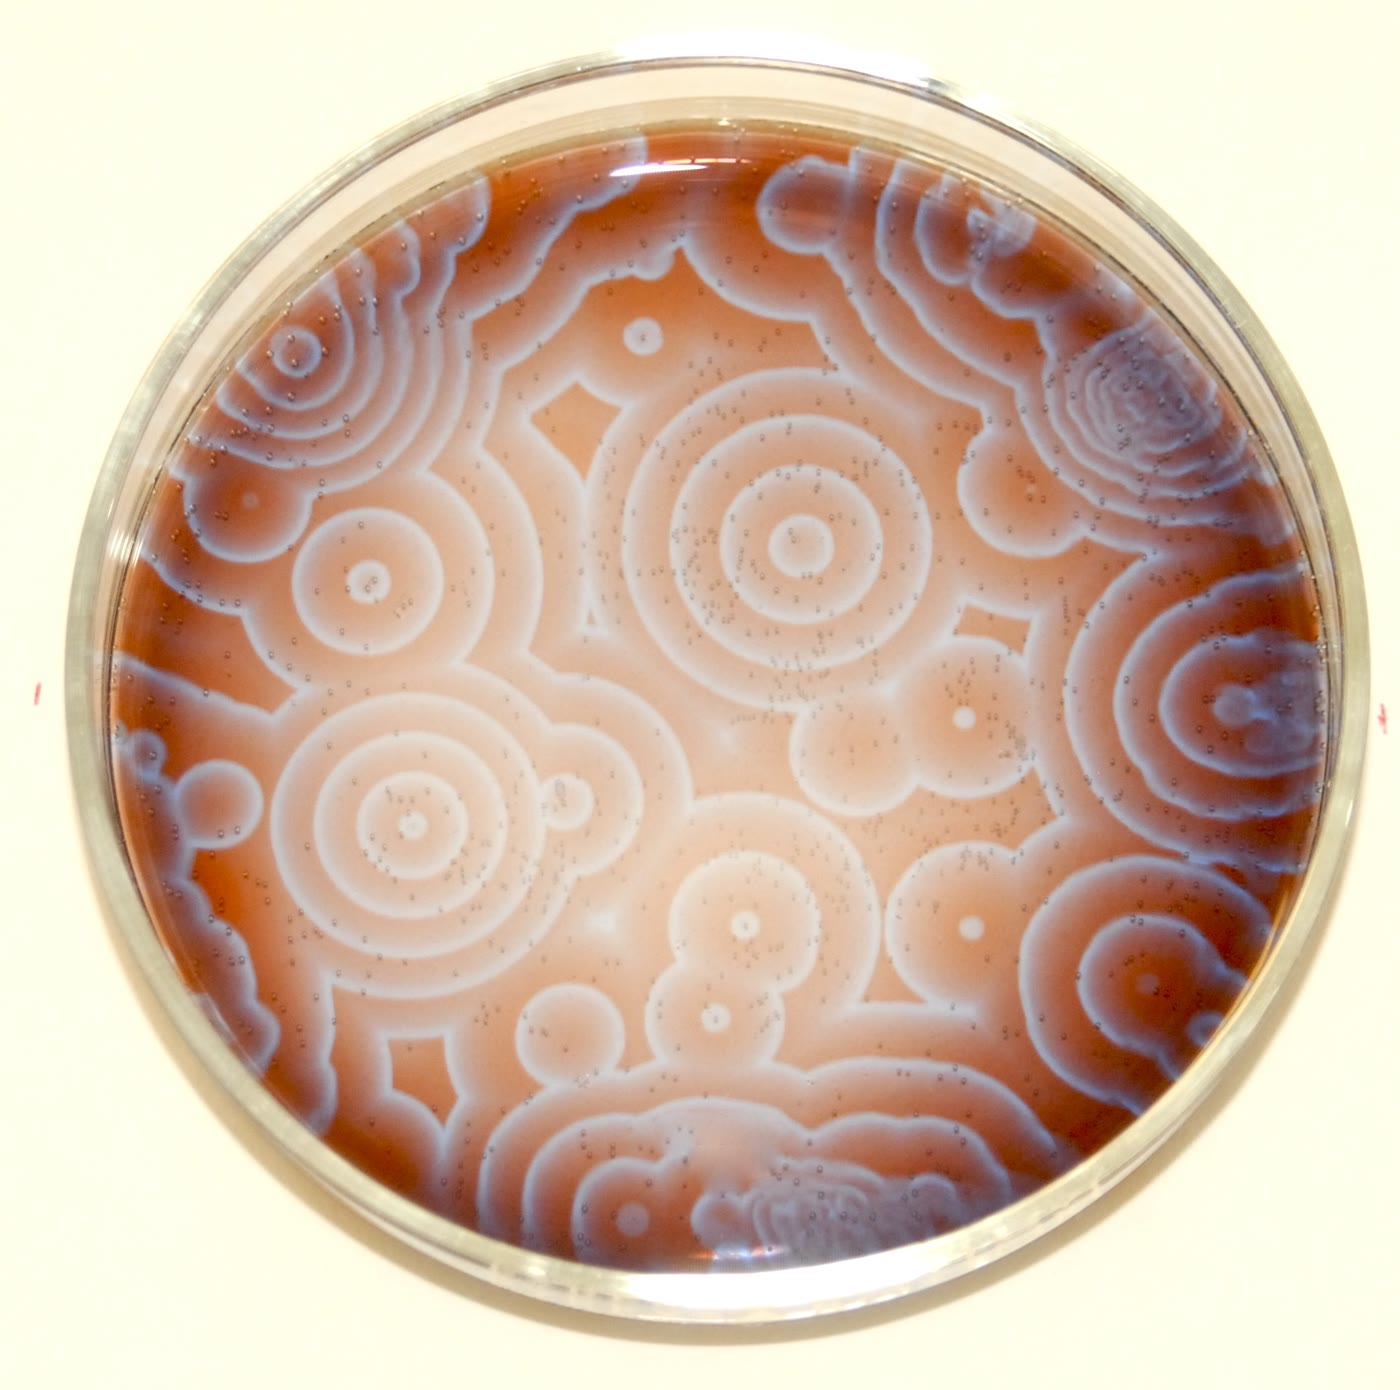
\includegraphics[width=0.48\linewidth]{images/book4/bz-reaction.jpg}

{\small موجات حلزونية لتفاعل بيلوسوف--جابوتنسكي في طبقة رقيقة من
المحلول: كل جبهة زرقاء موجة أكسدة للحفاز، تنتقل
في الوسط المختزل (الأحمر) ولا تستطيع أن تعود إلى المنطقة التي
غادرتها للتو.}
\end{omfigure}

\begin{definition}[طريقة الاسترخاء، زمن الاسترخاء الكيميائي]\label{def:b3:complex-kinetics:relaxation}
\emph{طريقة الاسترخاء}\index{طريقة الاسترخاء} تُحدث اضطرابًا مفاجئًا في نظام في
حالة توازن (بقفزة في درجة الحرارة أو الضغط أو المجال الكهربائي)
وتتتبع عودته إلى التوازن الجديد. ومن أجل اضطراب صغير يتناقص
الانحراف أسيًا، وفق \emph{زمن الاسترخاء
الكيميائي}\index{زمن الاسترخاء الكيميائي} $\tau$.
\end{definition}

\begin{proposition}[زمن استرخاء تفاعل تشارك]\label{prop:b3:complex-kinetics:relaxation-time}
من أجل $\mathrm{A + B \rightleftharpoons C}$ ($k_1$، $k_{-1}$)، بعد اضطراب صغير،
\[
  \frac1\tau = k_1([\mathrm A]_e + [\mathrm B]_e) + k_{-1} .
\]
\end{proposition}

\begin{proof}
لنكتب $[\mathrm C] = [\mathrm C]_e + x$، $[\mathrm A] = [\mathrm A]_e - x$، $[\mathrm B] = [\mathrm B]_e - x$. عندئذ $\dot x =
k_1([\mathrm A]_e - x)([\mathrm B]_e - x) - k_{-1}([\mathrm C]_e + x)$؛ والحدود الخالية من $x$ تتلاشى عند
التوازن، وبإهمال $x^2$: $\dot x = -[k_1([\mathrm A]_e + [\mathrm B]_e) + k_{-1}]x$.
\end{proof}

قياس $\tau$ عند عدة تراكيز يعطي مستقيمًا للمقدار $1/\tau$ بدلالة $[\mathrm A]_e +
[\mathrm B]_e$ ميله $k_1$ ومقطعه $k_{-1}$: أي الثابتين كليهما من تجارب
على نظام لا يبتعد أبدًا عن التوازن بأكثر من بضعة في المئة. وقد قاس مانفرد
آيغن بهذه الطريقة أسرع التفاعلات في المحلول، ومنها
تعادل \ce{H3O+} مع \ce{OH-}.

\begin{omfigure}
\begin{tikzpicture}
\begin{axis}[width=0.62\linewidth, height=5.0cm, xmin=0, xmax=780, ymin=0, ymax=1.05,
  axis lines=left, xlabel={\babelsublr{$t$ / \unit{\micro s}}}, ylabel={$([\mathrm C] - [\mathrm C]_e)/([\mathrm C]_0 - [\mathrm C]_e)$},
  tick label style={font=\small}, label style={font=\small},
  legend style={font=\scriptsize, draw=none, at={(0.97,0.97)}, anchor=north east},
  legend cell align=left]
\addplot[omDef, very thick] table[x=t_us, y=dC] {figdata/out/bachelor-3-chemical-relaxation.dat};
\addplot[omThm, thick, dashed] table[x=t_us, y=exp] {figdata/out/bachelor-3-chemical-relaxation.dat};
\legend{{\foreignlanguage{arabic}{معادلة السرعة الكاملة}}, {\babelsublr{$\eu^{-t/\tau}$, $\tau = \qty{156}{\micro s}$}}}
\draw[black!40, densely dotted] (axis cs:156,0) -- (axis cs:156,0.368) -- (axis cs:0,0.368);
\end{axis}
\end{tikzpicture}

{\small استرخاء $\mathrm{A + B \rightleftharpoons C}$ بعد قفزة في درجة الحرارة خفّضت
ثابت توازنه بنسبة 5\,\% (نموذج: $k_1 = \qty{1.0e8}{L.mol^{-1}.s^{-1}}$، $k_{-1} = \qty{1.0e3}{s^{-1}}$،
و\qty{1.0e-4}{mol/L} من A ومن B في المجموع): تتطابق معادلة السرعة الكاملة والدالة الأسية ذات
$1/\tau = k_1([\mathrm A]_e + [\mathrm B]_e) + k_{-1}$.}
\end{omfigure}

\begin{definition}[الجريان الموقوف، التحلل الضوئي الومضي]\label{def:b3:complex-kinetics:fast}
\emph{طريقة الجريان الموقوف}\index{طريقة الجريان الموقوف} تمزج محلولين
متفاعلين في نحو ميلي ثانية بدفعهما عبر خلاط إلى خلية
رصد، ثم توقف الجريان وتسجّل الامتصاصية أو
\omterm{def:b3:electronic-spectroscopy:luminescence}{التفلور}. و\emph{التحلل الضوئي الومضي}\index{تحلل ضوئي ومضي} يكوّن نوعًا
تفاعليًا بنبضة ضوئية قصيرة شديدة ويتتبع تفاعلاته بحزمة ضوئية
ثانية متأخرة.
\end{definition}

\begin{omfigure}
\begin{tikzpicture}[font=\small, >=Stealth]
  % two drive syringes
  \foreach \y/\lab in {1.1/A, -0.1/B}{
    \draw[thick] (0,\y) rectangle (2.2,\y+0.6);
    \fill[omDef!25] (0.6,\y+0.05) rectangle (2.15,\y+0.55);
    \draw[thick] (0.6,\y) -- (0.6,\y+0.6);
    \draw[thick] (-0.6,\y+0.3) -- (0.6,\y+0.3);
    \node at (1.4,\y+0.3) {\lab};
    \draw[thick] (2.2,\y+0.3) -- (2.8,\y+0.3);}
  \draw[thick] (2.8,1.4) -- (3.2,0.8) (2.8,0.2) -- (3.2,0.8);
  \node[draw, thick, circle, minimum size=5mm, fill=white] (mx) at (3.4,0.8) {};
  \node[font=\scriptsize, anchor=north] at (3.4,0.5) {\foreignlanguage{arabic}{خلاط}};
  \draw[thick] (mx.east) -- (4.4,0.8);
  \draw[thick, fill=omThm!15] (4.4,0.55) rectangle (5.4,1.05);
  \node[font=\scriptsize, anchor=north west, align=left] at (5.0,0.5) {\foreignlanguage{arabic}{خلية}\\ \foreignlanguage{arabic}{الرصد}};
  \draw[->, omThm, thick] (4.9,2.0) -- (4.9,1.1) node[pos=0, above, font=\scriptsize] {\foreignlanguage{arabic}{ضوء}};
  \draw[->, omThm, thick] (4.9,0.5) -- (4.9,-0.4) node[below, font=\scriptsize] {\foreignlanguage{arabic}{كاشف}};
  \draw[thick] (5.4,0.8) -- (6.2,0.8);
  \draw[thick] (6.2,0.5) rectangle (7.6,1.1);
  \draw[thick] (7.0,0.5) -- (7.0,1.1);
  \draw[thick] (7.0,0.8) -- (7.9,0.8);
  \draw[thick] (7.9,0.4) -- (7.9,1.2);
  \node[font=\scriptsize, anchor=south] at (6.9,1.15) {\foreignlanguage{arabic}{محقنة الإيقاف}};
  \draw[->, black!60] (-1.2,1.4) -- (-0.7,1.4) node[pos=0, left, font=\scriptsize] {\foreignlanguage{arabic}{الدفع}};
  \draw[->, black!60] (-1.2,0.2) -- (-0.7,0.2);
\end{tikzpicture}

{\small جهاز الجريان الموقوف. يدفع المحرّك محقنتين؛ فيلتقي المحلولان
في الخلاط ويملآن خلية الرصد في نحو ميلي ثانية؛ ثم
يصطدم مكبس محقنة الإيقاف بحاجز، فيتوقف الجريان، ويسجّل
الكاشف تفاعل المحلول الممزوج حديثًا.}
\end{omfigure}

\begin{omfigure}
\begin{tikzpicture}
\begin{axis}[width=0.62\linewidth, height=5.0cm, xmin=0, xmax=20, ymin=0, ymax=5.5,
  axis lines=left, xlabel={\babelsublr{$t$ / ms}}, ylabel={\babelsublr{$[\mathrm P_1]$ / \unit{\micro M}}},
  tick label style={font=\small}, label style={font=\small}]
\addplot[omDef, very thick] table[x=t_ms, y=P_uM] {figdata/out/bachelor-3-michaelis-menten-burst.dat};
\addplot[black!45, dashed, domain=0:20] {1.28 + 0.2*x};
\draw[->, black!60] (axis cs:4.5,0.7) -- (axis cs:0.25,1.24);
\node[font=\scriptsize, anchor=west] at (axis cs:4.5,0.7) {\foreignlanguage{arabic}{سعة الدفقة، \qty{1.28}{\micro M}}};
\end{axis}
\end{tikzpicture}

{\small منحنى دفقة في الجريان الموقوف (معطيات مسألة نهاية الأسبوع): يظهر الناتج
الأول \omterm{def:b3:complex-kinetics:enzyme}{لإنزيم} ذي خطوتين في دفقة سريعة يتبعها
مستقيم؛ والخط المتقطع يستكمل الحالة المستقرة رجوعًا إلى $t = 0$.}
\end{omfigure}

\begin{inthelab}[قياس بالجريان الموقوف]
تُملأ المحقنتان بمحلولي \omterm{def:b3:complex-kinetics:enzyme}{الإنزيم} والركيزة في المحلول المنظِّم
نفسه، وتُنظَّم حرارتهما، وتُطلقان عدة مرات لتنظيف الخلية قبل
الطلقات المسجَّلة؛ ويُؤخذ متوسط كل منحنى على خمس إلى عشر طلقات. 
والزمن الميت، أي عمر الخليط حين يبدأ الرصد، يُقاس مرة واحدة بتفاعل
معروف السرعة.
\end{inthelab}

\begin{safety}{\ghs[0.8cm]{GHS05}\ghs[0.8cm]{GHS06}\ghs[0.8cm]{GHS09}}
% ledger: ghs4:Br2
البروم: سائل متطاير كثيف أحمر بني؛ مميت إذا استُنشق، ويسبب
حروقًا شديدة، وسام جدًا للأحياء المائية. لا يُتداول إلا تحت ساحبة الأبخرة، بالقفازات
وواقٍ للوجه؛ ويُحتفظ بمحلول من ثيوكبريتات الصوديوم في المتناول لاختزال
ما ينسكب منه.
\end{safety}

\begin{history}[بودنشتاين وبيلوسوف]
قاس ماكس بودنشتاين وصموئيل ليند قانون سرعة الهيدروجين--البروم سنة
1906؛ وفسّره ينس كريستيانسن وكارل هيرتسفلد ومايكل بولاني سنة
1919 بالآلية المتسلسلة في هذا الفصل. ووجد بوريس بيلوسوف، عالم الكيمياء الحيوية في
موسكو، تفاعله المتذبذب نحو سنة 1951 وهو يبحث عن
نموذج كيميائي لدورة استقلابية؛ فرُفضت مخطوطته، ولم يُنشر إلا
ملخص قصير سنة 1959. وتناول أناتولي جابوتنسكي التفاعل في
الستينيات وفسّره؛ ثم وُضعت الآلية الكاملة في أوائل
السبعينيات.
\end{history}

\section{تمارين}

\begin{exercise}[$\star$]\label{exo:b3:complex-kinetics:1}
من أجل السلسلة $\ce{Cl2 -> 2 Cl}$، $\ce{Cl + H2 -> HCl + H}$، $\ce{H + Cl2 -> HCl + Cl}$، $\ce{2 Cl -> Cl2}$،
سمِّ كل خطوة \omterm{def:b3:complex-kinetics:chain}{وحوامل السلسلة}، واكتب التفاعل الإجمالي.
\end{exercise}

\begin{exercise}[$\star$]\label{exo:b3:complex-kinetics:2}
لنظام ليندمان $k_2 = \qty{1.0e7}{s^{-1}}$ و$k_{-1} = \qty{1.0e10}{L.mol^{-1}.s^{-1}}$ (معطيات
التمرين). احسب $[\mathrm M]_{1/2}$ والضغط الموافق عند \qty{750}{K}.
\end{exercise}

\begin{exercise}[$\star$]\label{exo:b3:complex-kinetics:3}
عبّر عن $v/V_{\max}$ عند $[\mathrm S] = K_M$ و$3K_M$ و$9K_M$. وأي تركيز يعطي 90\,\% من
$V_{\max}$؟
\end{exercise}

\begin{exercise}[$\star$]\label{exo:b3:complex-kinetics:4}
% ledger: enz:median.kcatKM, visc:H2O.25C
\omterm{def:b3:complex-kinetics:enzyme}{لإنزيم} $k_{\mathrm{cat}} = \qty{100}{s^{-1}}$ و$K_M = \qty{0.80}{mM}$. احسب ثابت نوعيته
وقارنه بحد الانتشار في الماء، \qty{7.4e9}{L.mol^{-1}.s^{-1}}،
وبالقيمة النموذجية $10^5$~\unit{L.mol^{-1}.s^{-1}}.
\end{exercise}

\begin{exercise}[$\star\star$]\label{exo:b3:complex-kinetics:5}
يُقترح أن التفكك $\ce{CH3CHO -> CH4 + CO}$ يجري عبر: $\ce{CH3CHO -> CH3 +
CHO}$ ($k_1$)؛ $\ce{CH3 + CH3CHO -> CH4 + CH3CO}$ ($k_2$)؛ $\ce{CH3CO -> CH3 + CO}$ ($k_3$)؛
$\ce{2 CH3 -> C2H6}$ ($k_4$). بيّن أن سرعة تكوّن الميثان هي
$k_2(k_1/2k_4)^{1/2}[\ce{CH3CHO}]^{3/2}$.
\end{exercise}

\begin{exercise}[$\star\star$]\label{exo:b3:complex-kinetics:6}
انطلاقًا من تركيزين متساويين من \ce{H2} و\ce{Br2}، مع $k' = 0.10$، بأي
عامل انخفضت السرعة حين يُستهلك نصف البروم؟ وكم من هذا
الانخفاض يعود إلى التثبيط؟
\end{exercise}

\begin{exercise}[$\star\star$]\label{exo:b3:complex-kinetics:7}
في خليط نموذجي من الهيدروجين والأكسجين (معطيات التمرين)، ثابت سرعة التفرع
$f = 1000\,p$، والإنهاء على الجدران $6000/p$ والإنهاء الثلاثي
$10\,p^2$، كلها بوحدة \unit{s^{-1}} مع $p$ بالكيلوباسكال. جد مجال الضغط الذي
ينفجر فيه الخليط.
\end{exercise}

\begin{exercise}[$\star\star$]\label{exo:b3:complex-kinetics:8}
السرعتان الابتدائيتان $\qty{0.20}{\micro M.s^{-1}}$ عند $[\mathrm S] = \qty{0.50}{mM}$ و$\qty{0.40}{\micro M.s^{-1}}$ عند
\qty{2.0}{mM}. جد $K_M$ و$V_{\max}$.
\end{exercise}

\begin{exercise}[$\star\star$]\label{exo:b3:complex-kinetics:9}
مع \qty{50}{\micro M} من مثبط، يلتقي مستقيم لاينويفر--بيرك \omterm{def:b3:complex-kinetics:enzyme}{لإنزيم}
($K_M = \qty{0.80}{mM}$) بالمستقيم غير المثبَّط على محور $1/v$ ويقطع محور
$1/[\mathrm S]$ عند \qty{-0.417}{mM^{-1}}. عيّن نوع التثبيط واحسب $K_i$.
\end{exercise}

\begin{exercise}[$\star\star\star$]\label{exo:b3:complex-kinetics:10}
من أجل $\mathrm{A + X \to 2\,X}$ مع $k = \qty{0.50}{L.mol^{-1}.s^{-1}}$، $a_0 = \qty{1.00}{mol/L}$ و$x_0 = \qty{0.010}{mol/L}$،
احسب الزمن الذي يكون فيه نصف الكمية النهائية من X حاضرًا، 
وزمن \omterm{def:b3:complex-kinetics:michaelis}{السرعة العظمى}.
\end{exercise}

\begin{exercise}[$\star\star\star$]\label{exo:b3:complex-kinetics:11}
من أجل البروسلاتور مع $A = 1$، احسب القيم الذاتية لمصفوفة جاكوبي عند
الحالة المستقرة من أجل $B = 1.5$ و$B = 2.5$، وصِف السلوك قرب
الحالة المستقرة في كل حالة.
\end{exercise}

\begin{exercise}[$\star\star\star$]\label{exo:b3:complex-kinetics:12}
من أجل $\mathrm{A + B \rightleftharpoons C}$ مع $k_1 = \qty{1.0e8}{L.mol^{-1}.s^{-1}}$ و$k_{-1} = \qty{1.0e3}{s^{-1}}$، 
و$[\mathrm A]_e = [\mathrm B]_e = \qty{2.70e-5}{mol/L}$، احسب $\tau$. وكيف تحصل على ثابتي السرعة كليهما
من قياسات الاسترخاء وحدها؟
\end{exercise}

\section{مسألة: إنزيم ومثبط وجرعة}

\begin{problem}[{مسألة نهاية الأسبوع --- إنزيم ومثبط وجرعة:
وسائط ميكايليس--منتن بالمربعات الصغرى، وثابت التثبيط لمثبط
تنافسي، والنشاط الباقي عند جرعة معينة، ودفقة في
الجريان الموقوف}]
\label{pb:b3:complex-kinetics:1}
% ledger: enz:median.kcatKM
يحلمه \omterm{def:b3:complex-kinetics:enzyme}{إنزيم} ($[\mathrm E]_0 = \qty{5.0}{nM}$ في الاختبارات) ركيزته؛ والسرعات الابتدائية
(معطيات المسألة):
\begin{center}\small
\begin{tabular}{lccccccc}
\hline
\babelsublr{$[\mathrm S]$ / mM} & 0.10 & 0.20 & 0.40 & 0.80 & 1.60 & 3.20 & 6.40 \\
\babelsublr{$v$ / \unit{\micro M.s^{-1}}} & 0.0566 & 0.0981 & 0.169 & 0.247 & 0.340 & 0.397 & 0.447 \\ \hline
\end{tabular}
\end{center}
بوجود مثبط، تعطي عمليات ضبط من النوع نفسه $V_{\max}$ دون تغيير 
و$K_M$ الظاهري: 0.79 و1.47 و2.38 و\qty{4.02}{mM} عند $[\mathrm I] = 0$ و20 و50 
و\qty{100}{\micro M}. وتعطي تجربة جريان موقوف مع $[\mathrm E]_0 = \qty{2.0}{\micro M}$ وركيزة مشبِعة
منحنى الدفقة في الشكل في القسم 5 (دفقة قدرها \qty{1.28}{\micro M}
بثابت سرعة \qty{625}{s^{-1}}، ثم \qty{200}{\micro M.s^{-1}}).

\medskip\noindent\textbf{الجزء الأول --- $K_M$ و$V_{\max}$.}
\begin{enumerate}
  \item لماذا تُستعمل السرعات الابتدائية؟
  \item ارسم منحنى لاينويفر--بيرك؛ يعطي مستقيم مربعاته الصغرى $K_M =
        \qty{0.773}{mM}$ و$V_{\max} = \qty{0.491}{\micro M.s^{-1}}$. أي النقاط تهيمن عليه؟
  \item لماذا يُفضَّل الضبط غير الخطي المباشر؟
  \item يعطي الضبط غير الخطي $K_M = 0.801 \pm \qty{0.023}{mM}$ و$V_{\max} = 0.502 \pm
        \qty{0.005}{\micro M.s^{-1}}$. هل تتوافق قيم لاينويفر--بيرك معها؟
  \item احسب $k_{\mathrm{cat}}$.
  \item احسب \omterm{def:b3:complex-kinetics:michaelis}{ثابت النوعية}.
  \item قارنه بحد الانتشار وبإنزيم نموذجي.
\end{enumerate}

\medskip\noindent\textbf{الجزء الثاني --- المثبط.}
\begin{enumerate}[resume]
  \item أي نوع من التثبيط تُظهره المعطيات؟
  \item اكتب $K_M^{\mathrm{app}}$ دالةً في $[\mathrm I]$.
  \item لمستقيم المربعات الصغرى للمقدار $K_M^{\mathrm{app}}$ بدلالة $[\mathrm I]$ المقطع \qty{0.799}{mM} 
        والميل \qty{0.0321}{mM.\micro M^{-1}}. استنتج $K_i$.
  \item خطؤه المعياري \qty{0.9}{\micro M}. أعطِ مجالًا بنسبة 95\,\% ($t = 4.30$ من أجل
        درجتي حرية).
  \item ماذا يقيس $K_i$؟
\end{enumerate}

\medskip\noindent\textbf{الجزء الثالث --- النشاط الباقي.}
\begin{enumerate}[resume]
  \item عبّر عن نسبة النشاط الباقي، $v_i/v_0$، دالةً في $[\mathrm S]$ 
        و$[\mathrm I]$.
  \item احسبها عند $[\mathrm S] = K_M$ و$[\mathrm I] = K_i$.
  \item عند $[\mathrm S] = K_M$ و$[\mathrm I] = 10K_i$.
  \item عند $[\mathrm S] = 10K_M$ و$[\mathrm I] = 10K_i$. علّق.
  \item بيّن أن تثبيطًا بنسبة 90\,\% عند $[\mathrm S] = K_M$ يقتضي $[\mathrm I] = 18K_i$.
  \item احسب هذا التركيز بقيمة $K_i$ المضبوطة.
\end{enumerate}

\medskip\noindent\textbf{الجزء الرابع --- الدفقة.}
\begin{enumerate}[resume]
  \item يعمل \omterm{def:b3:complex-kinetics:enzyme}{الإنزيم} على خطوتين، $\mathrm{E + S \to E{-}acyl + P_1}$ ($k_2$) ثم $\mathrm{E{-}acyl \to E +
        P_2}$ ($k_3$). لماذا يظهر $\mathrm P_1$ في دفقة؟
  \item سعة الدفقة $[\mathrm E]_0\bigl(k_2/(k_2 + k_3)\bigr)^2$. استنتج $k_2/(k_2 + k_3)$.
  \item من الميل المستقر، احسب $k_{\mathrm{cat}}$ وقارنه بالجزء الأول.
  \item ثابت سرعة الدفقة هو $k_2 + k_3$. استنتج $k_2$ و$k_3$.
  \item تحقق من أن $k_{\mathrm{cat}} = k_2k_3/(k_2 + k_3)$.
  \item اذكر النتيجة: تركيز المثبط الذي يعطي تثبيطًا بنسبة 90\,\% عند
        $[\mathrm S] = K_M$.
\end{enumerate}
\end{problem}
